%Provide an overview on how the user interface(s) of your system will 
%look like; if you have included this part in the RASD, you can simply refer to what you have 
%already done, possibly providing here some extensions if applicable.

The design of an intuitive yet expressive User Interface is important during the creation of the described application. The main activity of CKB is the development of source code both by students and educators, activity that is mainly carried out on computers rather than smartphones. Because of this, the target architecture for the final application is the computer. As indicated in the Requirement Analysis and Specification Document, there are two types of users (students and educators), requiring two different sets of functionalities. To keep these two sets separated, two User Interfaces are illustrated: a Student UI and an Educator UI. As reported in the Requirement Analysis and Specification Document, these representations are not meant to show the final product in details, but to provide a possible user interface along with the promise of the represented functionalities.
In particular:
\begin{itemize}
    \item 
    The Student UI must allow students to log in the system, visualize the badges won in all the tournaments they participated to, join new tournaments and see the ranking of all the opened and terminated tournaments. The UI must also allow students to join battles and invite other students to form a team. A Search option has been added to search for Tournaments and Students, allowing the visualizations of other students' badges.
    \item
    The Educator UI must allow educators to see all the tournaments created by them, displaying the actions performable for each one. It must display also the set of battles created in the contaxt of each tournament. Educators must be able to create battles and tournament, and to add personalized badges in new tournament. The interface for defining badges will be analyzed later.
\end{itemize}

\begin{figure}[H]
    \centering
    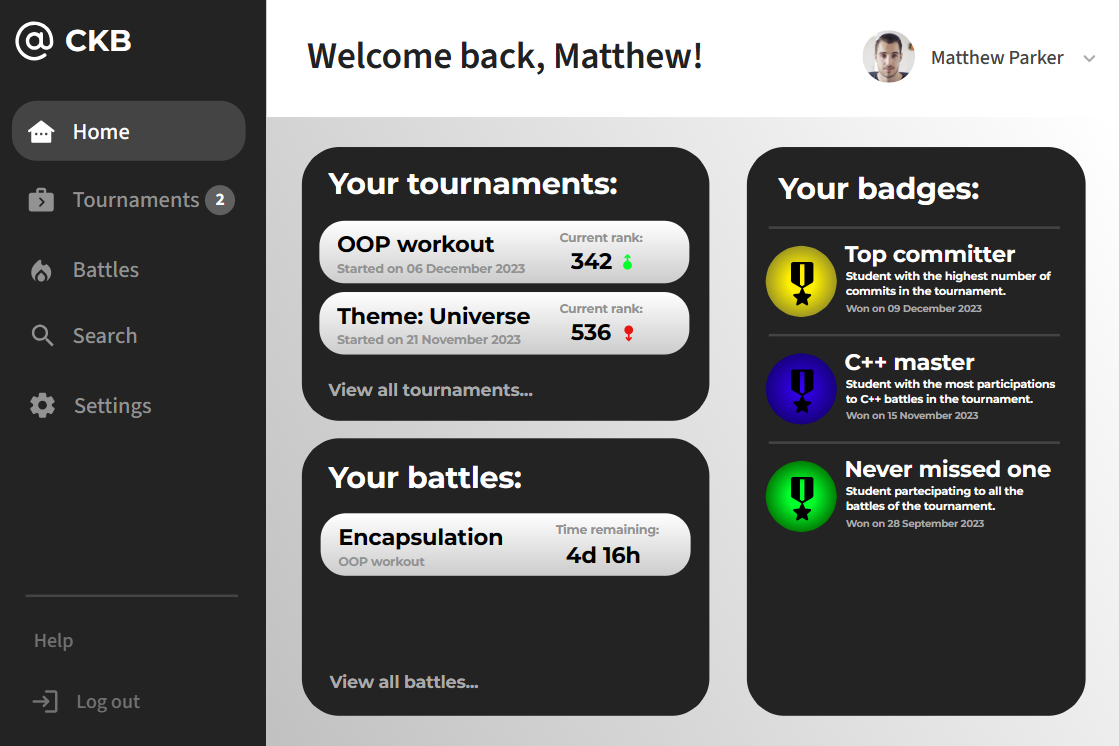
\includegraphics[width=0.8\linewidth]{Images/UI_Student_Home.png}
    \caption{Student Home screen}
    \label{fig:enter-label}
\end{figure}

\begin{figure}[H]
    \centering
    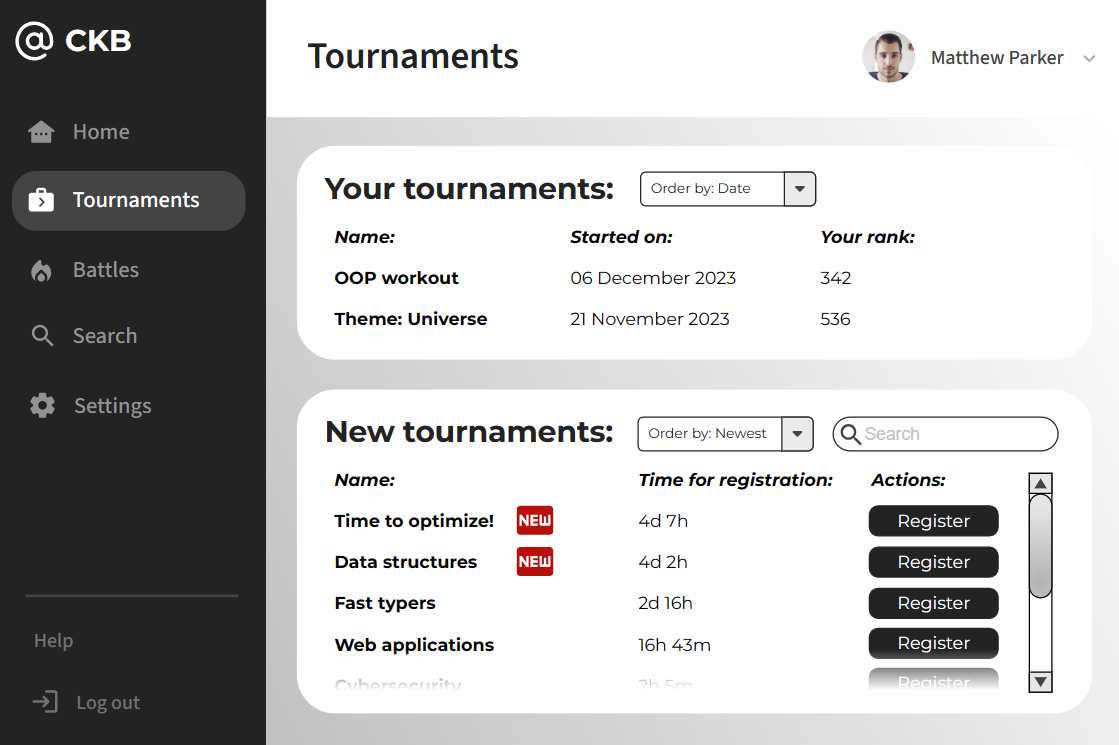
\includegraphics[width=0.9\linewidth]{Images/UI_Student_Tournaments.png}
    \caption{Student Tournaments screen}
    \label{fig:enter-label}
\end{figure}

\begin{figure}[H]
    \centering
    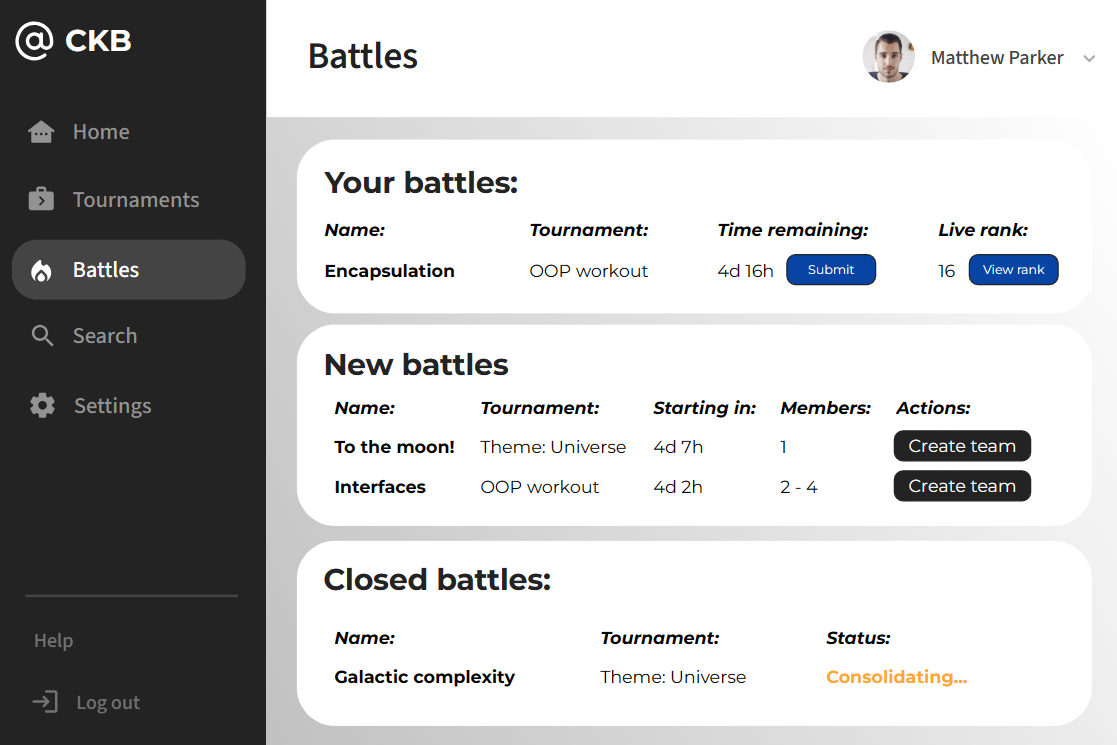
\includegraphics[width=0.9\linewidth]{Images/UI_Student_Battles.png}
    \caption{Student Battles screen}
    \label{fig:enter-label}
\end{figure}

\begin{figure}[H]
    \centering
    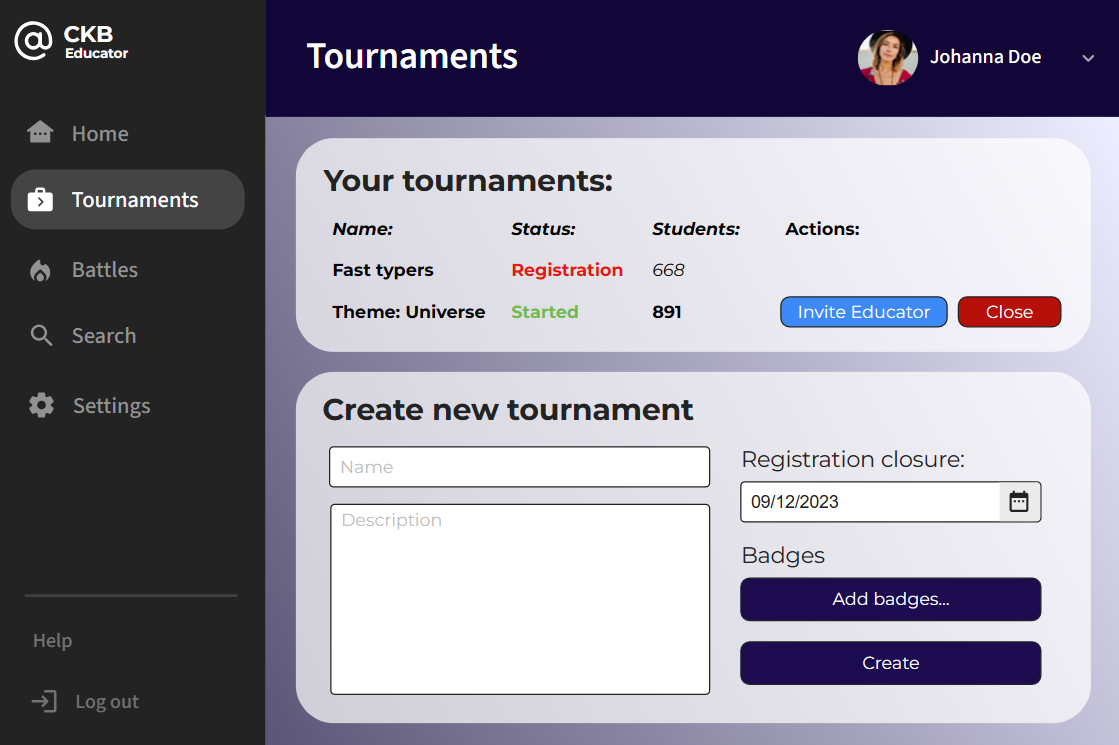
\includegraphics[width=0.9\linewidth]{Images/UI_Educator_Tournaments.png}
    \caption{Educator Tournaments screen}
    \label{fig:enter-label}
\end{figure}

\begin{figure}[H]
    \centering
    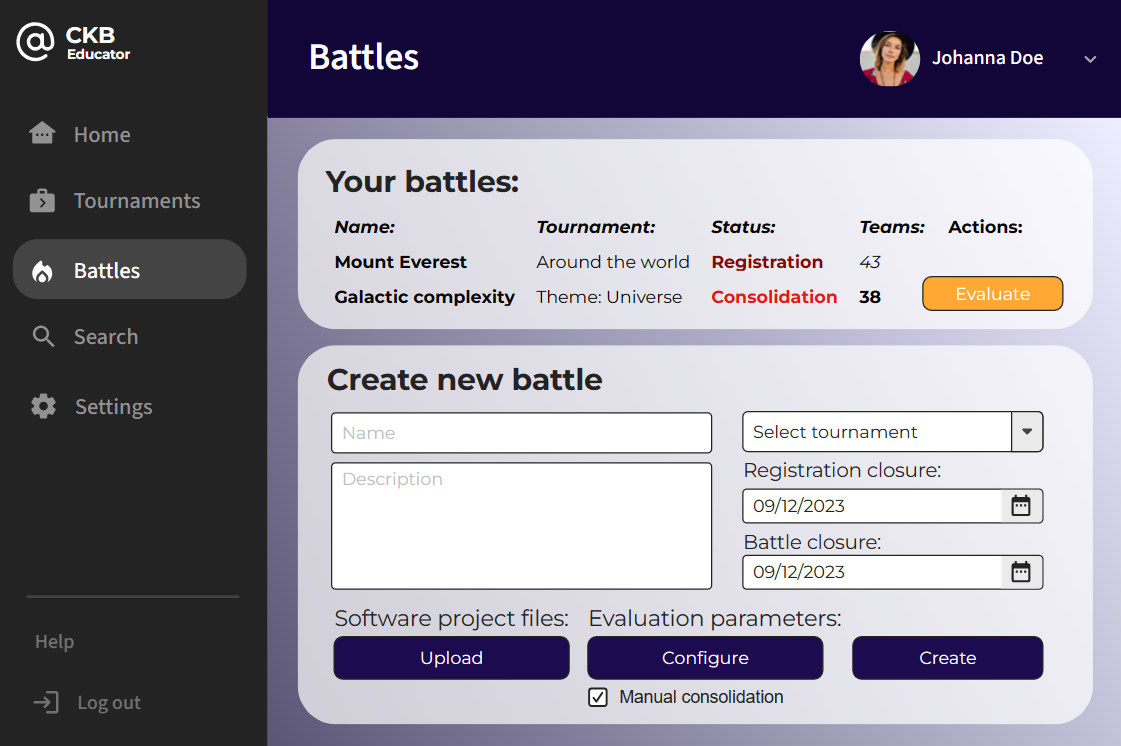
\includegraphics[width=0.9\linewidth]{Images/UI_Educator_Battles.png}
    \caption{Educator Battles screen}
    \label{fig:enter-label}
\end{figure}

\clearpage

To conclude the description of the User Interface, we present the interface offered to educators to define badges when creating a tournament, along with the specification of the rules that must be met by students in order to earn each badge. The variables on which the deserving students can be selected depend on the personal evaluation of the educator, and defining a closed set of variables and rules shared by all the educators limits the possible usage of a powerful mechanic such as gamification. On the other hand, defining a generic, powerful tool to define a wide range of filters, runs the risk of result in an interface too complicate for its common use, rendering the definition of simple, repetitive rules a tedious task. CodeKataBattle mitigates this issue by offering two ways of defining rules: one simple, intuitive way and one detailed and expressive way.\\
\\
The first modality of rule definition consists in a simple comparison between two variables: one referred to the individual performance of each student (student specific) and one referred either to the overall performance of all the student (global) or equal to a fixed constant. The terms of comparison between the two quantities are the ones applicable to two numeric parameters: $<,\leq,=,\neq,\geq,>$. The badge is then assigned to all the student whose specific variables satisfy the constraint (or the set of constraints). For example, assigning a badge to the student with the highest number of commits can be achieved in the following way:
\begin{figure}[H]
    \centering
    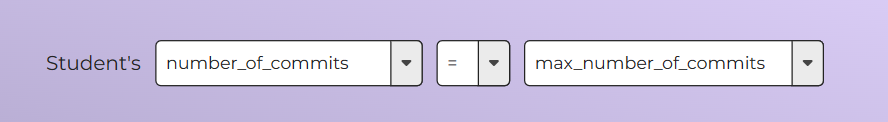
\includegraphics[width=0.9\linewidth]{Images/UI_Badge_form1.png}
    \caption{Student with maximum number of commits}
    \label{fig:UI_form1}
\end{figure}
As another example, assigning a badge to a student participating in all the battles in the tournament and reaching the first ten positions in the final tournament ranking can be performed in the following way:
\begin{figure}[H]
    \centering
    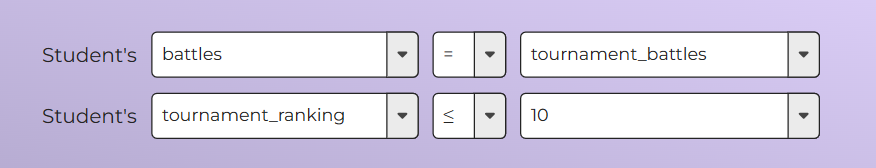
\includegraphics[width=0.9\linewidth]{Images/UI_Badge_form2.png}
    \caption{Student participating in all the battles and reaching the first ten positions in the tournament}
    \label{fig:UI_form2}
\end{figure}
The set of student variables, which will have a dedicated section explaining their meaning in the final application, is the following:

\begin{minted}{javascript}
    battles, //the number of battles in which the student participated
    battles_won, //the number of battles in which the student
                    //reached the first position in the final rank
    max_battle_ranking, //the maximum rank reached at the end of a battle
    max_commits, //maximum number of commits issued in a battle
    max_tournament_ranking, //the maximum rank reached during the tournament
    number_of_commits, //total number of commits issued by the student
    number_of_teammates, //total number of distinct teammates that
                        //participated with the student to the battles
    tournament_ranking, //the final rank of the student in the tournament
\end{minted}

The set of global variables, which will have a dedicated section explaining their meaning in the final application, is the following:

\begin{minted}{javascript}
    tournament_battles, //the number of battles in the tournament
    max_battles_won, //the maximum number of battles won
                    //by any student
    max_number_of_commits, //maximum number of commits issued by any student
    max_number_of_max_commits, //maximum number of commits issued
                                //by any student in a battle
\end{minted}

This set of predefined variables is not meant to be strictly closed and can be enriched during the development and maintaining of the system, along with a clear explanation of their meaning in a dedicated section.
\\
This form of rules is very intuitive and easy to use, but allows only for a restrict set of possible criteria for deciding whether assigning a badge or not. As a first step towards a more expressive interface, the system offers a way of defining new variables using JavaScript, specifying a function that returns a number starting from a wide dataset, which allows more complex informations to be taken into account. The informations offered to the educator are the following:
\begin{minted}{javascript}
tournament
    .startTime //timestamp of the beginning of the tournament
    //timestamps are expressed as second elapsed since 00:00:00 of 1/1/1970 UTC
    .finishTime //timestamp of the beginning of the tournament
    .students[] //array of students
        .email //email of the student
        .finalRank //final rank of the student
        .ranks[] //rank of the student at the end of each battle
                //regardless if the student participated or not
    .battles[] //array of battles
        .startTime //timestamp of the beginning of the battle
        .finishTime //timestamp of the ending of the battle
        .languages[] //programming languages of the battle
        .registeredStudents[] //array of student emails
        .teams[] //array of teams
            .members[] //emails of members of the team
            .rank //final position in the rank of the battle
            .commits[] //array of commits:
                       //the last entry is the final submission
                .timestamp //timestamp of the submission
                .language //programming language used
                .author //student email
                .text[] //lines of code
\end{minted}

All the educator has to do is define a function that uses the previous data to return a quantity: if the function describes a student specific variable, then the "student" object will be passed as a parameter. As an example, here is the process to describe the number of participations of each student in battles solvable with the programming language C\texttt{++}:

\begin{minted}{javascript}
function cpp_partecipations(student){
    let count = 0;
    for(let b of tournament.battles){
        if(b.registeredStudents.includes(student.email) && 
        b.languages.includes("C++")){
            count++;
        }
    }
    return count;
}
\end{minted}
After this, we can define a new global variable as the maximum number of participations in a C\texttt{++} battle by any student:

\begin{minted}{javascript}
function max_cpp_partecipations(){
    let max = 0;
    for(let s of tournament.students){
        let curr = cpp_partecipations(s);
        if(max < curr)
            max = curr;
    }
    return max;
}
\end{minted}
Once the two variables have been defined, the rule indicating the student with the most participations to C\texttt{++} battles can be expressed as above:

\begin{figure}[H]
    \centering
    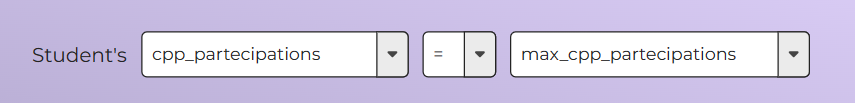
\includegraphics[width=0.9\linewidth]{Images/UI_Badge_form3.png}
    \caption{Student with the most participations to C\texttt{++} battles}
    \label{fig:UI_form3}
\end{figure}
We note that the scripts proposed by the educators will be executed in the same controlled environment as the student submissions, and badges with incorrect descriptions will be discarded.\\
\\
To add yet another layer of expressiveness, the system allows educators to define a rule function that directly returns if a student is eligible for a certain badge or not. To make a final example, here is the rule for selecting the students that issued two commits in less than a minute:

\begin{minted}{javascript}
function two_commits_one_minute(student){
   for(let b of tournament.battles){
      for(let t of b.teams){
         if(t.members.includes(student.email)){
            for(let i=0; i<t.commits.length-1; i++){
               for(let j=i+1; j<t.commits.length &&
               t.commits[j].timestamp - t.commits[i].timestamp < 60; j++){
                  if(t.commits[i].author == student.email &&
                  t.commits[j].author == student.email){
                     return true;
                  }
               }
            }
         }
      }
   }
   return false;
}
\end{minted}
These are all the options that an educator has to describe the rules for assigning badges to students. The system offers both a simple, intuitive way to assign badges to students based on simple parameters and a more complex, expressive way of defining detailed rules. The scripts used for defining rules can be saved to be reused and shared among educators and many of them are offered as templates to make the draft of complex rules more intuitive, along with removing the strict need for educators to eventually learn JavaScript in depth just for this purpose.